\documentclass[11pt]{article}
%%%%%%%%%%%%%%%%%%%%%%%%%%%%%%%% Algunos Paquetes Necesarios 
\usepackage{fancyhdr, graphicx, wrapfig,lipsum}
\usepackage[utf8]{inputenc}% Language
\usepackage{pgf,tikz,pgfplots}
\usepackage[spanish]{babel}
\usepackage{xcolor}
\usepackage{mathrsfs}
\usetikzlibrary{arrows}
\pagestyle{empty}
\usepackage[margin=1in]{geometry} % Margins														
\usepackage{amssymb}
\usepackage{multicol}
\usepackage{amsmath, amsthm, amsfonts}
\usepackage{longtable} % Table accross multiple pages
\usepackage{hyperref}  % Use Hyperlinks
\usepackage{enumitem} % Reduce space in enumerate
\usepackage{txfonts}
\usepackage{float}
\usepackage{lipsum}
\usepackage{fancybox}
\usepackage[pangram]{blindtext}
\usepackage{tcolorbox}
\usepackage[framemethod=TikZ]{mdframed}



\begin{document}
	
	\newcommand{\myDoc}{Tarea 1}
	\newcommand{\myDate}{Primer semestre 2022}
	\newcommand{\myCourse}{Laboratorio Avanzado}
	\newcommand{\myName}{Rubí Esmeralda Ramírez Milián}
	\newcommand{\myCarnet}{201804565}
	\newcommand{\degre}{\ensuremath{^\circ}}
	\newcommand{\R}{\mathbb{R}}
	\newcommand{\F}{\mathbf{F}}
	\newcommand{\vi}{\mathbf{\hat{i}}}
	\newcommand{\vj}{\mathbf{\hat{j}}}
	\newcommand{\vk}{\mathbf{\hat{k}}}
	%%%%%%%%%%%%%%%%%%%%%%%%%%%%%%%%%%%%%%%Fancyboxes
	
	
	\newcounter{problem}[section]\setcounter{problem}{0}
	\renewcommand{\theproblem}{%\arabic{section}.
		\arabic{problem}}
	
	\newenvironment{problem}[1][]{%
		\refstepcounter{problem}
		
		\ifstrempty{#1}%
		% if condition (without title)
		{\mdfsetup{%
				frametitle={%
					\tikz[baseline=(current bounding box.east),outer sep=0pt]
					\node[anchor=east,rectangle,fill=purple!20]
					{\strut Problema~\theproblem};}
			}%
			% else condition (with title)
		}{\mdfsetup{%
				frametitle={%
					\tikz[baseline=(current bounding box.east),outer sep=0pt]
					\node[anchor=east,rectangle,fill=purple!20]
					{\strut Problema~\theproblem:~#1};}%
			}%
		}%
		% Both conditions
		\mdfsetup{%
			innertopmargin=10pt,linecolor=pink!40,%
			linewidth=2pt,topline=true,%
			frametitleaboveskip=\dimexpr-\ht\strutbox\relax%
		}
		\begin{mdframed}[]\relax%
			\label{#1}}{\end{mdframed}}
	
	
	\newcounter{solution}[section]\setcounter{solution}{0}
	\renewcommand{\thesolution}{%\arabic{section}.
		\arabic{solution}}
	\newenvironment{solution}[2][]{%
		\refstepcounter{solution}%
		\ifstrempty{#1}%
		{\mdfsetup{%
				frametitle={%
					\tikz[baseline=(current bounding box.east),outer sep=0pt]
					\node[anchor=east,rectangle,fill=green!20]
					{\strut Soluci\'on~\thesolution};}}
		}%
		{\mdfsetup{%
				frametitle={%
					\tikz[baseline=(current bounding box.east),outer sep=0pt]
					\node[anchor=east,rectangle,fill=green!20]
					{\strut Soluci\'on	~\thesolution:~#1};}}%
		}%
		\mdfsetup{innertopmargin=10pt,linecolor=green!20,%
			linewidth=2pt,topline=true,%
			frametitleaboveskip=\dimexpr-\ht\strutbox\relax
		}
		\begin{mdframed}[]\relax%
			\label{#2}}{\end{mdframed}}
	
	%%%%%%%%%%%%%%%%%%%%%%%%%%%%%%%%%%% Tema - BEGIN
	\newtheoremstyle{Tema}% name of the style to be used
	{5mm}% measure of space to leave above the theorem. E.g.: 3pt
	{3mm}% measure of space to leave below the theorem. E.g.: 3pt
	{}% name of font to use in the body of the theorem
	{}% measure of space to indent
	{\bfseries}% name of head font
	{\newline}% punctuation between head and body
	{20mm}% space after theorem head
	{}% Manually specify head
	
	\theoremstyle{Tema} \newtheorem{Tema}{Tema} %%%%% Template para Temas
	\theoremstyle{Tema} \newtheorem{serie}{Serie}              %%%%%  Template para Series de ejercicios
	\theoremstyle{Tema} \newtheorem{ejercicio}{Ejercicio}    %%%%%  Template para Ejercicios
	%%%%%%%%%%%%%%%%%%%%%%%%%%%%%%%%%%% Tema - END
	
	
	%%%%%%%%%%%%%%%%%%%%%%%%%%%%%%%%%%% Encabezado - BEGIN %%%%%%%%%%
	\fancypagestyle{firststyle}
	{
		\renewcommand{\headrulewidth}{1.5pt}
		\fancyhead[R]{
			\textbf{Universidad de San Carlos de Guatemala} \\
			\textbf{Escuela de Ciencias F\'isicas y Matem\'aticas}\\
			\textbf{\myName}\\
			\textbf{\myCourse }\\
			\textbf{\myCarnet}    %%%%%%%%%% Agregar nombre del curso 
			%%%%%%%%%%%%%%%%%%%%%% Agregar fecha en formato: Enero 15, 2015
		}
		\fancyhead[L]{ 
			%\includegraphics[height=1.6 cm, width=5.5 cm]{LogoColor}  
		}
	}
	%%%%%%%%%%%%%%%%%%%%%%%%%%%%%%%%%%% Encabezado - END %%%%%%%%%%
	
	%%%%%%%%%%%%%%%%%%%%%%%%%%%%%%%%%%% Encabezado (pagina 2 en adelante) - BEGIN %%%
	\fancypagestyle{allStyle}
	{
		\renewcommand{\headrulewidth}{0.8 pt}
		\fancyhead[R]{
			\emph{\myDoc $-$ \myCourse} %%%% Modificar n\'umero de examen parcial y nombre del curso
		}
		\fancyhead[L]{}  
		\fancyfoot[C]{}
		\fancyfoot[R]{\thepage}
	}
	%%%%%%%%%%%%%%%%%%%%%%%%%%%%%%%%%%% Encabezado (pagina 2 en adelante) - END %%%
	
	\date{}
	\setlength{\headheight}{0.65 in} % fixes \headheight warning
	%%%%%%%%%%%%%%%%%%%%%%%% BEGIN%%%%%%%%%%%%%%
	
	\pagestyle{allStyle}
	
	\thispagestyle{firststyle}
	%%%%%%%%%%%%%%%%%%%%%%%%%%%%%%%%% Titulo - BEGIN
	\begin{center}
		\LARGE
		\textsc{\myDoc}\\\normalsize % Modificar el N\'umero del examen parcial
		\medskip
		\hrule height 1.8pt
	\end{center}
	
	
	%	\section*{Instrucciones:}Resuelva esta tarea en su cuaderno u hojas dejando constancia de sus procedimientos. Sus respuestas deben estar escritas y encerradas en un cuadro a lapicero.
	
	
	
	\begin{problem}
		Compile, corra y analice el funcionamiento de los códigos:

			\begin{itemize}
				\item sizes.cpp
				\item inter.cpp
			\end{itemize}
		
	\end{problem}
	
	\begin{itemize}
		\item \textbf{sizes.cpp:}
		\subitem Compilar y correr:
		
		\begin{figure}[H]
			\centering
			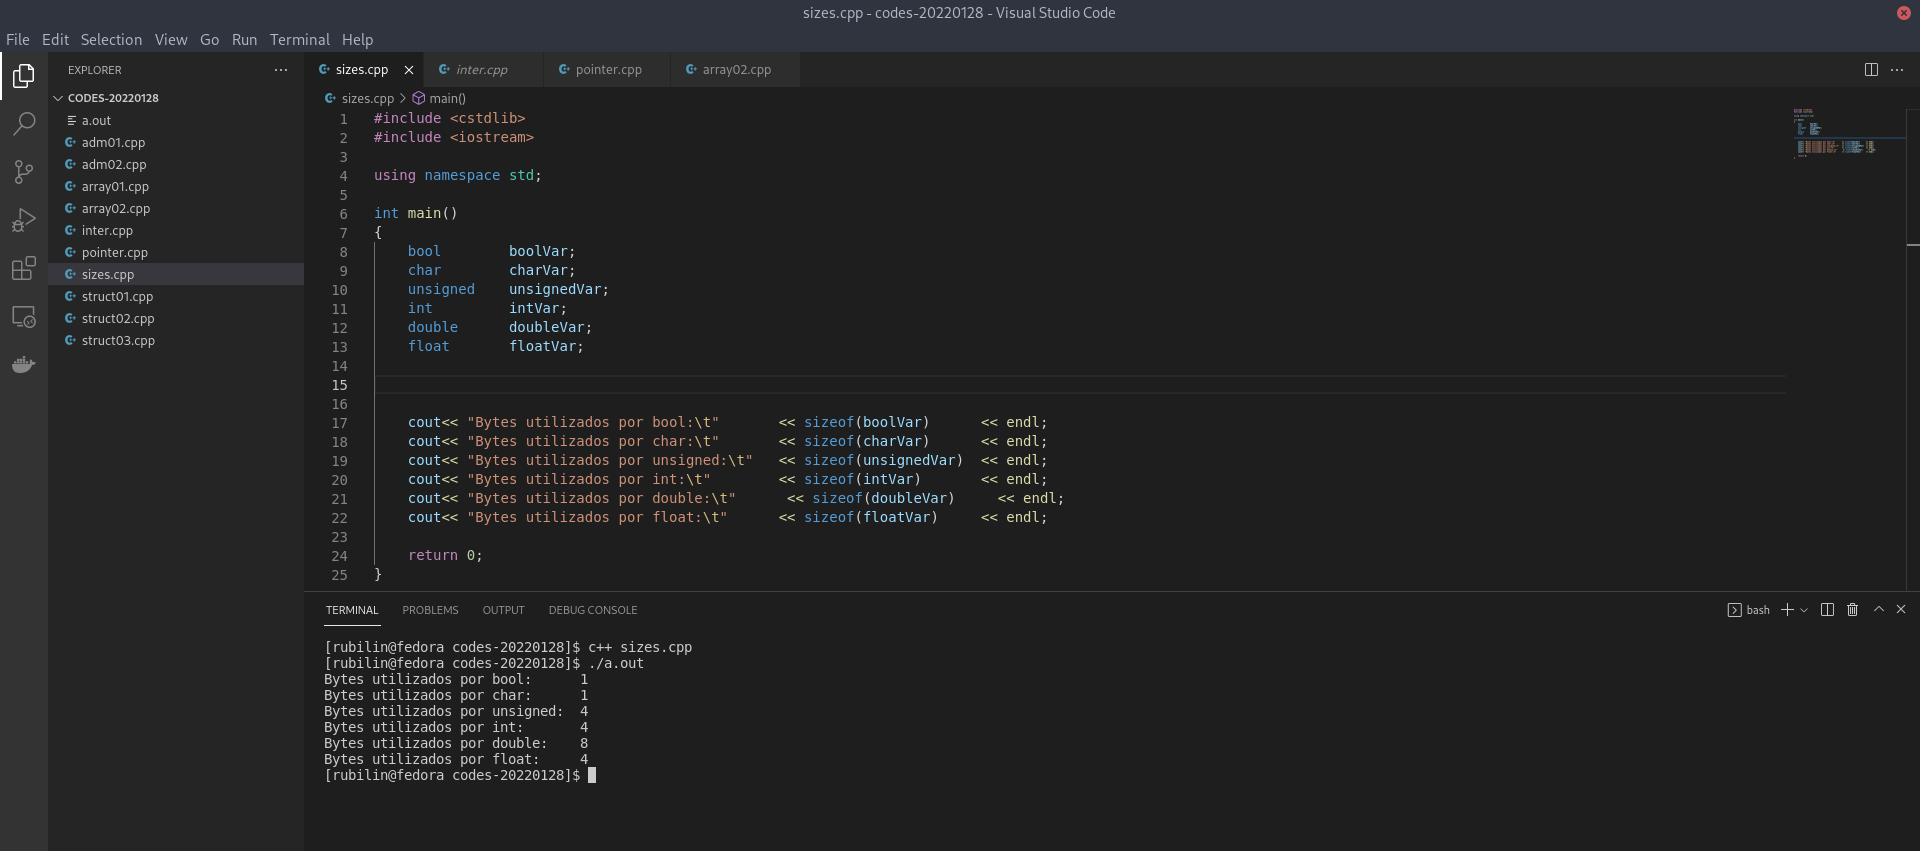
\includegraphics[width=0.7\linewidth]{img1.png}
			\caption{Resultado de  correr sizes.cpp}
			\label{fig:img1}
		\end{figure}
		
		
	\subitem	Las primeras dos líneas se llaman a las librerías que se van a utilizar, la primer cstdlib  contiene los prototipos de funciones de C para gestión de memoria dinámica, control de procesos y otras. Y iostream que es utilizado para operaciones de entrada/salida. Luego se utiliza los namespace std para dar acceso al espacio de nombres (namespace) std, donde se encuentra encerrada toda la librería estándar.
	
	En el main, se define tipos de varibles, una variable booleana, un caracter, un número sin signo, un entero, una varible double y un floatante o valor real. Y con la ayuda de  <<cout>> se imprime en consola un string se deja una espacio tabular y luego se utiliza la función <<size of>> la cual indica el tamaño de la variable a la que se le aplica. En los casos de las variable booleanas y caracteres su tamño es de 1 byte. Las variables sin signo, los enteros y los floatantes tienen un tamaño de 4 bytes. Y las variables double como su nombre lo indican tiene el doble que son 8 bytes.
		
		
		
		\item \textbf{inter.cpp}
		
		\subitem Compilar y correr:
		\begin{figure}[H]
			\centering
			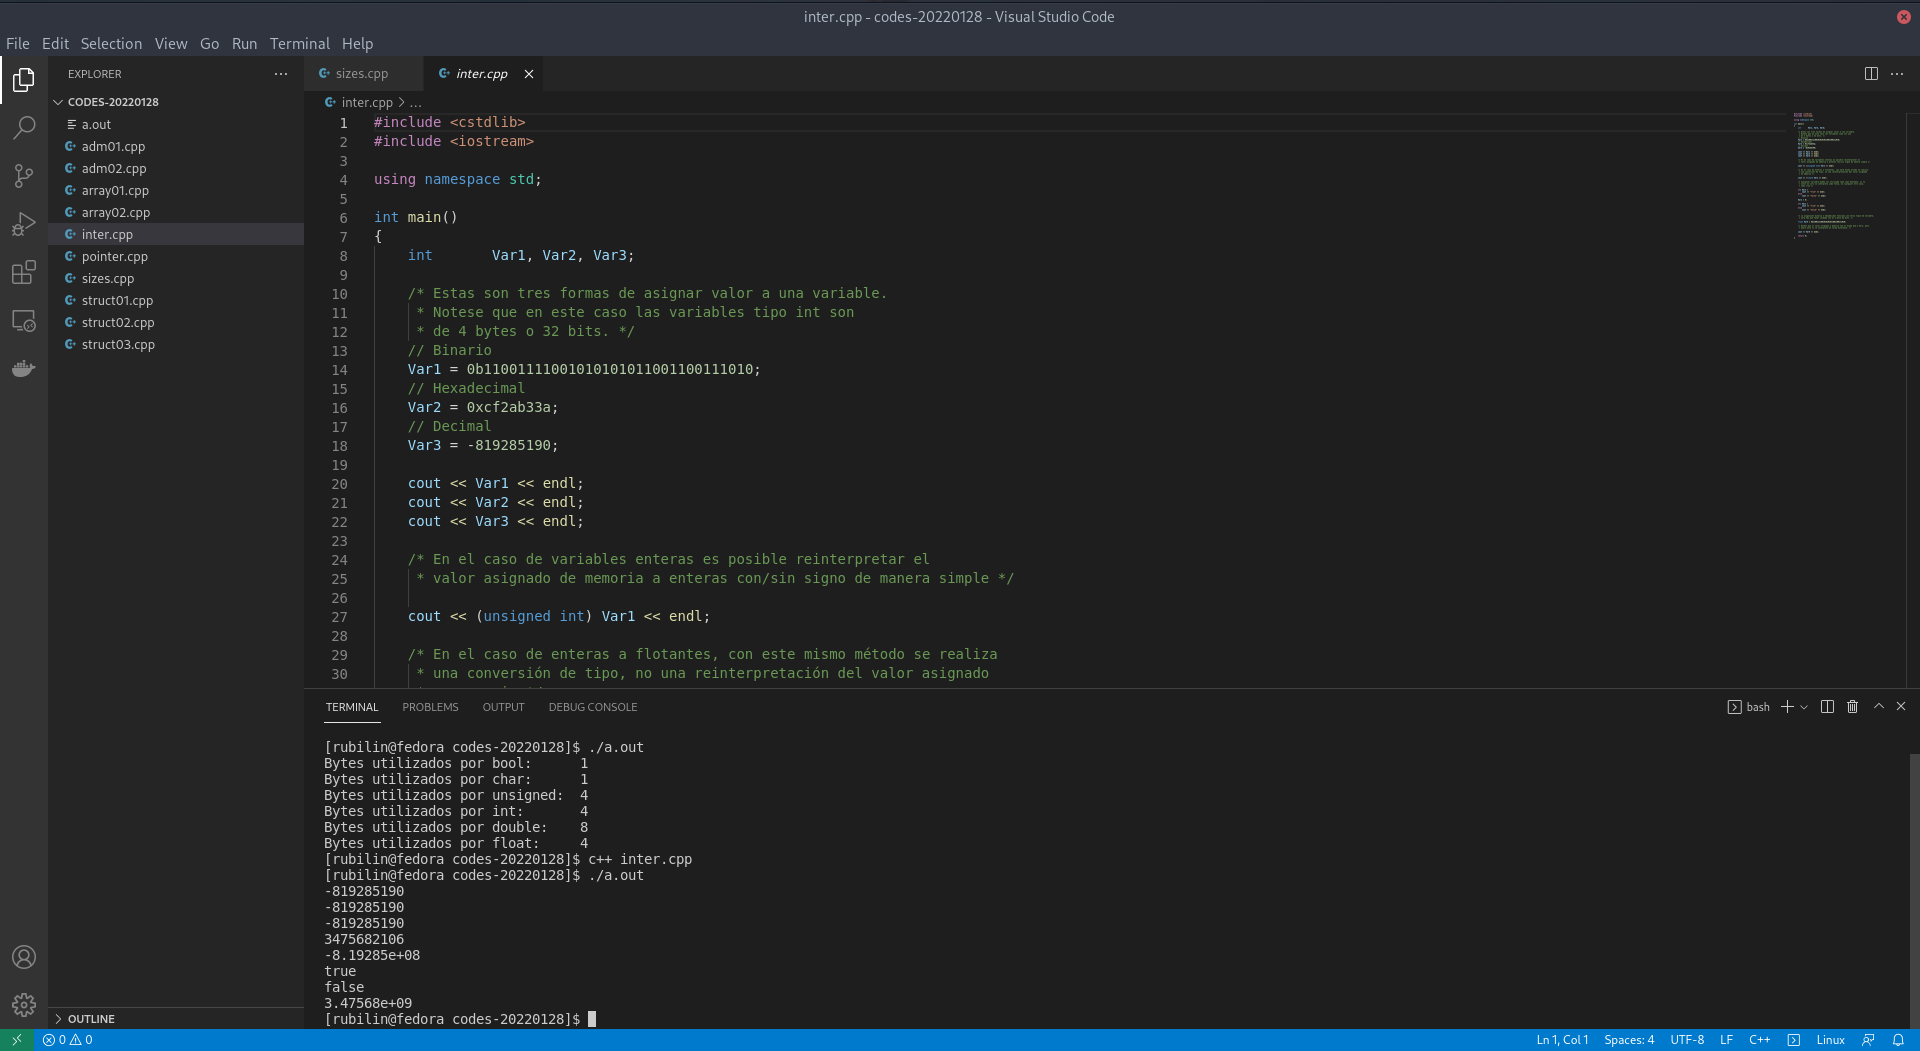
\includegraphics[width=0.7\linewidth]{img2.png}
			\caption{Resultado de correr inter.cpp}
			\label{fig:img2}
		\end{figure}
		
		
		\subitem	Las primeras dos líneas se llaman a las librerías que se van a utilizar, la primer cstdlib  contiene los prototipos de funciones de C para gestión de memoria dinámica, control de procesos y otras. Y iostream que es utilizado para operaciones de entrada/salida. Luego se utiliza los namespace std para dar acceso al espacio de nombres (namespace) std, donde se encuentra encerrada toda la librería estándar.
		
		
		En la función main primero se declaran tres variables de tipo entero y luego se les asigna el mismo valor <<-819285190>> pero de tres formas diferentes una para cada varible, de forma binaria con <<0b>> en complemento a dos, de forma hexagesimal <<0x>>, y de forma decimal. Y luego se imprimen en consola. 
		
		En la siguiente línea, en caso de variables enteras  se  hace una reinterpretación de la variable <<Var1>> a entero sin signo  por lo que cambia a  $2^{32}-819285190=3475682106$ y se imprime. Luego en el caso de flotantes se hace una conversión de tipo flotante (no una reinterpretación del valor asignado) y de nuevo se imprime.
		
		Luego, se utilizan las variables enteras y flotantes se pueden utilizar como variables booleanas utilizando la condición if y else. Si la variable es cero se interpretará como <<false>> si no se interpretará como <<true>>. Como al principio la variable <<Var1>> tenía un valor no igual a cero se imprimió <<true>> y luego como se le asignó el valor 0 y por ende se imprimió <<false>>.
		
		Luego se declara la cuarta variable <<Var4>> de tipo flotante y se le asigna el mismo valor en binario que a la varibale <<Var1>>. Al imprimirlo se puede notar que se interpreta de forma diferente, sin signo, se interpreta como $2^{32}-819285190=3475682106$ pero escrito de formato de coma flotante $3.47568e+09$
		
		
		
		
	\end{itemize}
	
	
	
	
	
	
	
	
	
	
	
	
	
	
	
	
	
	
	\begin{problem}
		Investigue la representación binaria con complemento a 2 para
		números enteros negativos. Calcule la representación a 32 bits
		de los siguientes números: -125, -4096, -1000000.
	\end{problem}
	
	\textbf{Complemento a 2}: Es una operación matemática en números binarios, es usado como un método de cómputo en la representación de  números con signo\cite{Compleme27:online}.
	

	El complemento a dos de un número $N$ que, expresado en el sistema binario con $n$ dígitos, se define como:
	
	$${\displaystyle C_{2}^{N}=2^{n}-N}$$
	
	
	El total de números positivos será ${\displaystyle 2^{n-1}-1}$ y el de negativos ${\displaystyle 2^{n-1}}$, siendo $n$ el número máximo de bits. El 0 contaría aparte\cite{Compleme27:online}.
	
	 
	  Para obtener el complemento a dos de un número se puede primero pasar al complemento a uno ( el valor obtenido al invertir todos los bits en la representación binaria del número, intercambiando 0 por 1 y viceversa)  y luego sumar 1, debido a que el complemento a dos de un número binario es  	una unidad mayor que su complemento a uno (por la representación duplicada del 0) \cite{Compleme27:online}, \cite{Compleme58:online}.
	
	$${\displaystyle C_{2}^{N}=C_{1}^{N}+1}$$	
	
	
	
	\begin{itemize}
		\item \textbf{-125}:
		\begin{itemize}
			\item Resolver para el entero sin signo: $(125)_{10}=(1111101)_2$
			
			\item Rellenar con ceros para formar un número de 32-bit: 
			
			$0000$ $0000$ $0000$ $0000$ $0000$ $0000$ $0111$ $1101$
			
			\item Para un número negativo debemos invertir todos los bits:
			
			1111 1111 1111 1111 1111 1111 1000 0010
			
			\item Sumar uno:
			
			1111 1111 1111 1111 1111 1111 1000 0011
			
			
		\end{itemize}
		
		
		
		\item \textbf{-4096}:
		\begin{itemize}
			\item Resolver para el entero sin signo: $(4096)_{10}=(1 0000 0000 0000)_2$
			
			\item Rellenar con ceros para formar un número de 32-bit: 
			
			$0000$ $0000$ $0000$ $0000$ $0001$ $0000$ $0000$ $0000$
			
			\item Para un número negativo debemos invertir todos los bits:
			
			1111 1111 1111 1111 1110 1111 1111 1111
			
			\item Sumar uno:
			
			1111 1111 1111 1111 1111 0000 0000 0000
		
			
			
		\end{itemize}
		
		
			
		\item \textbf{-1000000}:
		\begin{itemize}
			\item Resolver para el entero sin signo: $(1000000)_{10}=(1111 0100 0010 0100 0000)_2$
			
			\item Rellenar con ceros para formar un número de 32-bit: 
			
			$0000$ $0000$ $0000$ $1111$ $0100$ $0010$ $0100$ $0000$
			
			\item Para un número negativo debemos invertir todos los bits:
			
			1111 1111 1111 0000 1011 1101 1011 1111
			
			\item Sumar uno:
			
			1111 1111 1111 0000 1011 1101 1100 0000
			
			
			
		\end{itemize}
		
		
	\end{itemize}
	
	
	\nocite{BinaryNu62:online}
	
	\bibliographystyle{ieeetr}% otras opciones {plain}
	\bibliography{referencias}
	
	%%%%%%%%%%%%%%%%%%%%%%%%%%%%%%%%% Instrucciones - BEGIN
	
	\vspace{0.1 in}
	
\end{document} %%%%%%%%%%%%%%%%%%%%%%%% BEGIN%%%%%%%%%%%%%%